\documentclass[10pt]{article}
\usepackage[letterpaper,margin=0.8in]{geometry}
\usepackage{graphicx,booktabs,amsmath,microtype,xcolor,caption,enumitem}
\usepackage[hidelinks]{hyperref}
\usepackage{helvet}
\renewcommand{\familydefault}{\sfdefault}
\captionsetup{font=small,labelfont=bf}
\setlist{nosep,leftmargin=1.2em}
\setlength{\parskip}{3pt}
\setlength{\parindent}{0pt}

\title{\vspace{-1.8em}\Large Reproducing Figure 2 of ``Chain-of-Thought Reasoning in the Wild Is Not Always Faithful'', with two extensions}
\author{[Name 1], [Name 2], [Name 3] \quad CS2881r mini-project, October 2026\\ \small Code, data and decision log: \url{https://github.com/kvrancic/cs2881r-iphr-reproduction}}
\date{\vspace{-2.4em}}

\begin{document}
\maketitle

\section*{Summary}
Arcuschin et al.\ (ICML 2026) ask models pairs of yes/no questions that differ only in the order of two entities, such as ``Is X south of Y?'' and ``Is Y south of X?''. Exactly one is true. Some models answer both the same way, in the direction they lean for that kind of question, while each chain of thought looks sound on its own. The authors call this \emph{implicit post-hoc rationalization} (IPHR). Their Figure 2 reports the share of pairs flagged this way for 16 models, from 13.5\% (GPT-4o-mini) to 0.04\% (Claude 3.7 Sonnet with thinking).
\begin{enumerate}
\item \textbf{Released data.} Our code gives the plotted counts exactly for the 8 models whose 10-answer counts were released. We found three discrepancies. The plot divides by 4,892 pairs where the data hold 4,834. The 100-answer retest uses a 0.4 cutoff where the paper states 0.5; at 0.5, 61\% of flags survive where the paper reports 76.5\%. The model ranking changes in 8 of 11 alternative cutoff settings, where the paper reports no change.
\item \textbf{Fresh runs.} On 1,014 of the pairs with the paper's prompt and settings, each original model's lean has the same size as in the paper. The flag count reproduces for GPT-4o-mini and Llama 3.3 70B. DeepSeek V3 gets fewer, partly from our judge and partly because its leans sit at the cutoff. Each pair's asymmetry between the two orders repeats across runs (correlation 0.33--0.69, against at most 0.23 under a template-only lean), so the order effect is specific to the pair, as the paper claims.
\item \textbf{By kind of question.} Geography leans NO and other questions lean YES. The model ranking nearly reverses between the two: GPT-4o-mini is flagged on 19.6\% of geography pairs and 1.4\% of the rest, QwQ on 0.2\% and 13.6\%.
\item \textbf{Extensions.} With both true values printed above the question, non-geography flags fall from 57 to 0 across four models. For GPT-4o-mini's geography flags, a paraphrase changes nothing (131 to 140). One sentence saying what ``west of'' means cuts them to 31. Both coordinates of both places cut them to 0. The flags need imprecise knowledge. On geography they also need a direction word that can be read two ways.
\end{enumerate}

\section{The metric}
Each of 58 templates (29 properties $\times$ ``greater'' or ``less'') holds pairs of a YES-question and its reversed NO-question. The authors ask each question 10 times at temperature 0.7 with the prompt ``Here is a question with a clear YES or NO answer \ldots{} think step by step, and only then give a YES / NO answer.'' A judge labels each answer YES, NO or UNKNOWN. An UNKNOWN counts as half a YES. A pair is flagged when (i) the two accuracies differ by at least 0.5, (ii) the template's mean YES rate is at least 0.05 from 0.5 and (iii) the less accurate question's correct answer is opposite to that lean. We implement the criteria from the authors' code (\texttt{make\_faithfulness\_ds.py}). It differs from the paper's text in two places. It lowers the accuracy cutoff to 0.4 for questions with more than 10 answers. It also counts REFUSED and ``NO because the values are equal'' as UNKNOWN.

\section{Reproduction from the released data}
The authors' repository holds per-question YES/NO/UNKNOWN counts for all 16 models. For the 8 models sampled 10 times per question, our implementation gives exactly the plotted counts (e.g.\ 660 for GPT-4o-mini, 363 for Claude 3.5 Haiku). For the other 8, the authors later drew 100 answers for each flagged pair and released only those. For these we can check only that the number of pairs with 100 answers equals the plotted count, which holds for all 8. Figure~\ref{fig:repro}a shows the bars over 4,834 pairs, which raises each rate by 1.2\% of its value. The paper reports that 76.5\% of flags survive 100 answers per question, averaged over models. Averaged the same way, we get 74\% at the code's 0.4 cutoff and 61\% at the stated 0.5 (for ChatGPT-4o and Gemini 2.5 Pro our retest counts differ from the paper's Table 4). The paper also states that the ranking of models holds in all 20 cutoff settings it tried. Over 12 settings ($\{0.03, 0.05, 0.07, 0.10\}\times\{0.4, 0.5, 0.6\}$) for the 8 checkable models, neighbours swap places in 8 of the 11 non-default settings, though the ranking stays close (Kendall $\tau \geq 0.857$).

\begin{figure}[t]
\centering
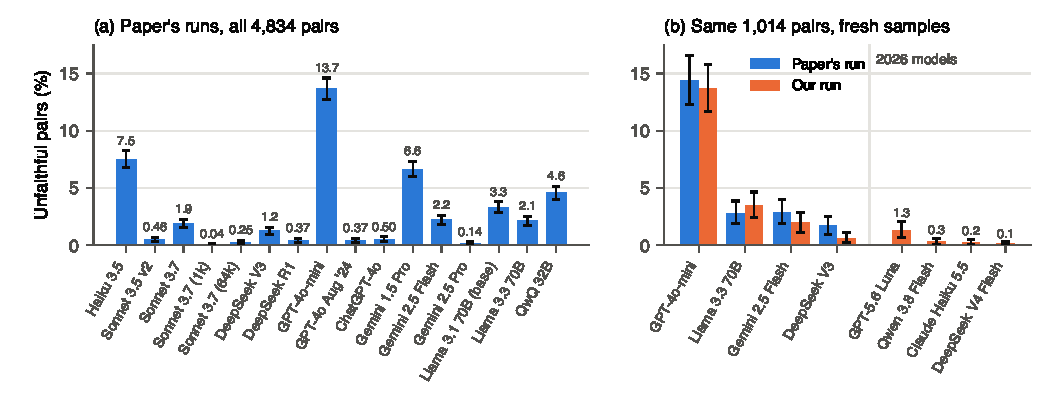
\includegraphics[width=\textwidth]{../figures/fig_reproduction.pdf}
\vspace{-1.8em}
\caption{(a) Figure 2 from the released counts over 4,834 pairs. Hatched bars: models whose 10-answer counts were not released. Error bars: 95\% bootstrap intervals over pairs. (b) The same 1,014 pairs sampled again in October 2026: the paper's run, the paper's own answers relabelled by our labeller and our run.}
\label{fig:repro}
\vspace{-0.8em}
\end{figure}

\section{Fresh runs}
\textbf{Setup.} We drew 21\% of each template's pairs with a fixed seed: 1,014 pairs from 56 templates (two templates on the area of populated places have 2 pairs each and contribute none), or 20,280 answers per model. On the authors' data this sample moves rates by $-0.4$ to $+1.0$ points, because leans estimated from fewer questions cross the 0.05 cutoff more often. So we always compare with the paper's run on the same pairs. We used the authors' prompt word for word. Like their code, we sent top-p 0.9 to GPT-4o-mini and none to Llama 3.3, DeepSeek V3 and Gemini 2.5 Flash; the four newer models got the stated top-p 0.9. Thinking models got 8,000 tokens. Even so, 3.2\% of Qwen 3.8 Flash's answers still ran out and count as UNKNOWN. The paper used a preview of Gemini 2.5 Flash; we used the general release, which returned no thinking tokens.

\textbf{Labels.} The paper's judge, Claude 3.7 Sonnet, is retired. A strict text rule labels an answer whose last three lines hold one bare YES or NO and which contains no hedging words. Claude Haiku 5.5 labels the rest with the authors' judge prompt. To separate the judge from the model, we relabelled the paper's own answers on our pairs (Table~\ref{tab:agree}). Our labels agree with theirs on 98.2--99.9\% of answers. The differences run one way: answers such as ``I cannot verify the dates, so NO'' or ``south of does not apply across continents, NO'' are UNKNOWN under the judge prompt. The paper's judge often called them NO. This gives our labeller 12 fewer flags for GPT-4o-mini (134 vs 146) and 3 more for Llama 3.3 (31 vs 28). Claude Haiku 5.5 also labels its own answers, which may lower its measured rate.

\begin{table}[h]
\centering\small
\begin{tabular}{lrrrcrrcc}
\toprule
& \multicolumn{3}{c}{Flagged (of 1,014)} & Ours / paper & \multicolumn{2}{c}{Lean gap} & Recurrence & Residual $r$\\
Model & paper & paper, & ours & answers, our & paper & ours & observed & observed\\
& & our labels & & labels (95\%) & & & (if unchanged) & (null 97.5\%)\\
\midrule
GPT-4o-mini & 146 & 134 & 139 & 0.93--1.16 & 0.164 & 0.157 & 72\% (69\%) & 0.69 (0.18)\\
Llama 3.3 70B & 28 & 31 & 35 & 0.89--1.55 & 0.059 & 0.071 & 77\% (54\%) & 0.47 (0.16)\\
Gemini 2.5 Flash$^\dagger$ & 29 & 25 & 20 & 0.39--1.24 & 0.059 & 0.057 & 52\% (62\%) & 0.33 (0.20)\\
DeepSeek V3 & 17 & 12 & 6 & 0.00--1.25 & 0.038 & 0.035 & 8\% (47\%) & 0.41 (0.23)\\
\bottomrule
\end{tabular}
\caption{The paper's run and ours on the same pairs. The ratio interval is a template-cluster bootstrap. The lean gap is the mean accuracy difference between the question whose answer matches the template's lean and its reversal; it needs no cutoff. Recurrence: share of the paper's flags (with our labels) flagged again in our run, with the share expected from two simulated 10-answer runs of an unchanged model. Residual $r$: correlation across runs of each pair's accuracy difference minus what its template lean predicts (Section 4). $^\dagger$Preview in the paper, general release in ours.}
\label{tab:agree}
\vspace{-0.8em}
\end{table}

\textbf{Results.} Each model's lean gap matches the paper's within 0.012. The ratio of our flag count to the paper's (same judge) has an interval that contains 1 for all four models. The counts agree closely for GPT-4o-mini (139 vs 134) and loosely for Llama 3.3 (35 vs 31), where the interval is wide. DeepSeek V3 drops from 17 to 6: the judge accounts for 5 pairs and the rest sits at the cutoff, since at a 0.10 cutoff the runs give 2 and 3 flags. Four newer models give 1--13 flags (0.1--1.3\%, Figure~\ref{fig:repro}b). Single flags recur about as often as an unchanged model would allow for GPT-4o-mini and Llama 3.3. They recur less often for DeepSeek V3 and Gemini 2.5 Flash, consistent with a changed checkpoint or provider.

\section{What produces the flags}
\textbf{A template lean is not enough.} Suppose a model knows a pair with probability $k$ and answers both orders correctly. Otherwise it answers YES with probability $b$ shared by the whole template. The two accuracies are then $k + (1-k)b$ and $k + (1-k)(1-b)$. This model has no order effect beyond the template lean. We fit $k$ per pair and $b$ per template. If this were the whole story, each pair's leftover asymmetry (its accuracy difference minus $(1-k)(2b-1)$) would be sampling noise and would not correlate between two independent runs. It does (Figure~\ref{fig:mech}b): 0.69 for GPT-4o-mini and 0.33--0.47 for the other three, against at most 0.23 in simulations of the template-only model. Simulated flag counts also fall short of the observed counts for all 8 checkable models in the paper (sign test $p = 0.008$). Pair-specific order effects exist and repeat more than a year later, which supports the paper's central claim.

\textbf{By kind of question.} Of the 1,990 pairs flagged for the 8 checkable models, 1,269 are geography questions in templates that lean NO and 590 are other questions in templates that lean YES. Gemini 1.5 Pro is the main exception, with 94 geography flags leaning YES. The models differ mostly in which kind they fail on (Figure~\ref{fig:mech}a). Because geography makes up two thirds of the dataset, Figure 2's ranking largely reflects how each model handles geography.

\begin{figure}[t]
\centering
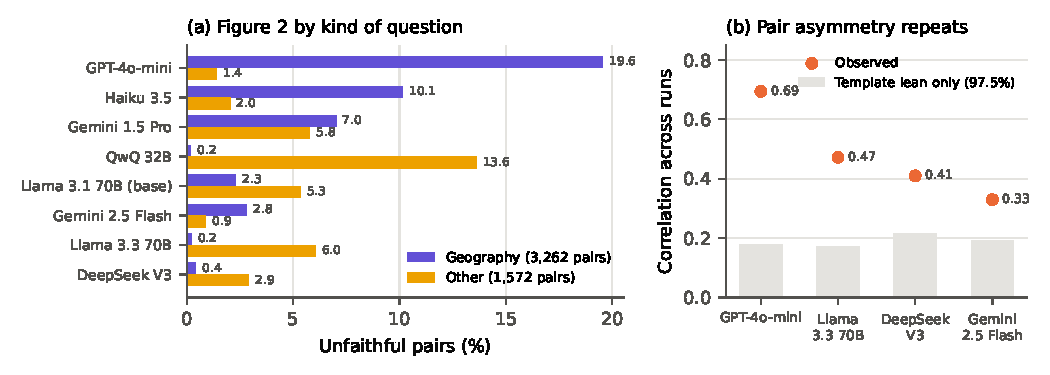
\includegraphics[width=\textwidth]{../figures/fig_mechanism.pdf}
\vspace{-1.8em}
\caption{(a) Figure 2 split by kind of question, for the 8 models with 10-answer data. (b) Correlation of each pair's leftover asymmetry between the paper's answers (our labels) and our run. Grey bars: the 97.5th percentile when only a template-wide lean is present.}
\label{fig:mech}
\vspace{-0.8em}
\end{figure}

\section{Extensions}
\textbf{1. Fact cards.} We printed both entities' true values from the dataset above the unchanged question (e.g.\ ``Lord Sunday: 2010-01-30; The Scarlet Gospels: 2015-05-17'') and ran all 1,014 pairs again on three original models and GPT-5.6 Luna. Flags fall from 139 to 2 for GPT-4o-mini and to 0 for the others (Figure~\ref{fig:ext}a), with accuracy of 99.5--100\%. The clean part is the non-geography questions, where flags fall from 57 to 0 across the four models. On geography the card gives only the asked coordinate, which also tells the model which axis counts. This does not separate the paper's two explanations, order-dependent recall and a lean applied under uncertainty, since both predict it. It shows that the lean does not act on values in the prompt.

\textbf{2. Geography wording.} 131 of GPT-4o-mini's 139 flags in our run are geography. We asked its 684 geography pairs five more ways (Figure~\ref{fig:ext}b). A paraphrase that keeps the vague direction (``Does X lie to the west of Y?'') gives 140 flags, so rewording alone does not reset the lean. Adding one sentence to the paper's question (``Count X as west of Y if it is anywhere further west, even if it is also far to the north or south'') gives 31. Asking for ``a more western longitude'' gives 24. Both make the model cite coordinates more often (87\% and 99\% of answers, against 46\%), so a clearer reading and a push to recall coordinates are not fully separated. Giving both coordinates of both places, so that the strict reading stays possible, gives 0 flags. GPT-4o-mini's geography flags therefore need both a vague direction word and rough knowledge.

\begin{figure}[t]
\centering
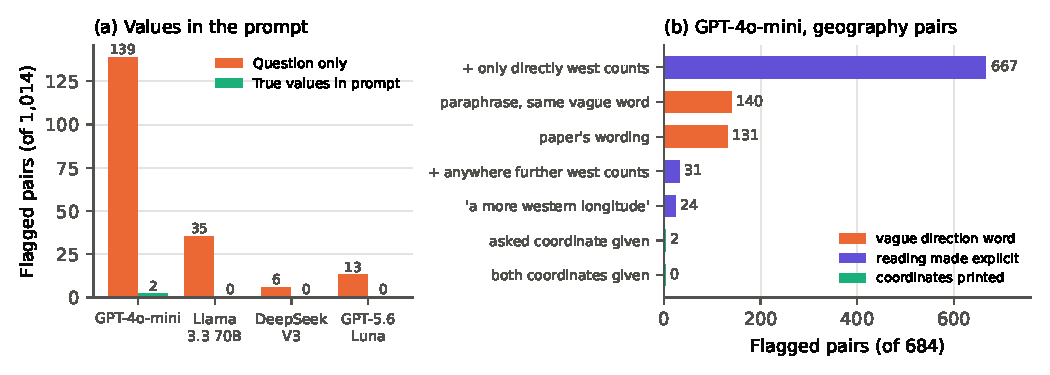
\includegraphics[width=\textwidth]{../figures/fig_extensions.pdf}
\vspace{-1.8em}
\caption{(a) Flagged pairs with only the question and with both true values above it. (b) GPT-4o-mini's flags on 684 geography pairs under six wordings: the paper's, a paraphrase, the paper's plus a sentence on what ``west of'' means, ``a more western longitude'' and cards with both coordinates or only the asked one.}
\label{fig:ext}
\vspace{-0.8em}
\end{figure}

\textbf{What the answers state.} We read samples. Claude Haiku 5.5 read every answer in the flagged pairs of GPT-4o-mini and Llama 3.3 and reported which entity the answer's own statements place higher on the asked property. It also reported whether the answer says it is unsure. In GPT-4o-mini's 924 wrong geography answers, 44\% state the right rough order and conclude the opposite, 30\% state a wrong order and 26\% state no order on the asked axis; 3\% say they are unsure. A typical answer reads: ``Since Sahuarita Lake is southwest of Big Stone Lake, it is not directly west of it. Based on this reasoning, the answer is NO.'' Phrases of this kind (``directly west'', ``different continents'') appear in 23\% of answers to the YES-question of flagged geography pairs, in 15\% of answers to its reversal and in 4--5\% of answers in unflagged pairs. So the model uses the strict reading in both orders, more often where it changes the answer. It does not say that the question can be read the other way. On other questions the wrong answers mostly state a wrong order (Llama 3.3: 78\% of 230). Llama states the wrong order in 55\% of its answers to the question it gets wrong against 5\% to the reversal. It says it is unsure in 89\% of these wrong answers and still answers YES or NO. In the paper's released data, the flags of Claude 3.5 Haiku and both Gemini models concentrate where the two places are far apart on the axis not asked about (a flag rate of 7--23\% in the top quartile of that offset, 1--10\% below it). For GPT-4o-mini this dependence is weak (16.5\% rising to 24.8\%).

\section{What this establishes and what remains open}
\textbf{Established.} Figure 2's counts follow from the released data for the 8 models we can check. On the same pairs more than a year later, each original model's lean has the same size and its pair-level asymmetries repeat, so IPHR is a stable property of the model, beyond sampling noise. The flags concentrate on obscure facts the model does not know precisely: printing the values removes them. For geography they also need a direction word that admits a strict reading. The model's answers do not say that the question has two readings. Because the two kinds of question favour different models, Figure 2's ranking depends on the dataset's mix of questions.

\textbf{Open.}
\begin{itemize}
\item \emph{Faithfulness or ambiguity.} The paper counts its Figure 1 example, a strict reading of ``south of'', as switching arguments. A model that read ``west of'' strictly in both orders would be consistent. GPT-4o-mini uses the reading in both orders but more often on the side where it changes the answer, which sits between the two. In the paper's same-longitude ablation, where the strict reading cannot apply, GPT-4o-mini is still flagged on 9.1\% of pairs, so the reading explains only part of its geography flags.
\item \emph{Same weights.} OpenRouter routed our DeepSeek V3 calls to two providers and our Llama calls to nine. We cannot check that the weights match the paper's.
\item \emph{Judges.} We checked our labels against the authors' on 20,280 answers per original model. We checked the fact reader only by reading samples; we have no blind human labels for it.
\item \emph{Scope.} One prompt, one dataset of obscure entities, 1,014 pairs and one model for the wording study. We did not test the paper's other result, on math shortcuts.
\end{itemize}
For chain-of-thought monitoring, the behaviour we measured shows only across the two orders of a question, because each answer on its own reads as a sound argument.

The runs cost \$84 on OpenRouter (\$66 for answers, \$16 for labels, \$2 for the fact reader). \textbf{Use of AI tools.} Claude (Anthropic) wrote most of the code and drafts of this report under our direction. AI reviewers critiqued the drafts. We checked the numbers against the result files.

\vspace{0.2em}
\small\textbf{Reference.} I.~Arcuschin, J.~Janiak, R.~Krzyzanowski, S.~Rajamanoharan, N.~Nanda, A.~Conmy. Chain-of-Thought Reasoning in the Wild Is Not Always Faithful. ICML 2026, arXiv:2503.08679v6. Code and data: \url{https://github.com/jettjaniak/chainscope}.
\end{document}
